\input{sty/mybeamerstyle.tex}
%\input{data/ipdata.txt}

\usepackage{booktabs}%, makecell}
\usepackage{overpic}
\usepackage{multirow}
\usepackage{makecell}

\usepackage{hhline}
\usepackage{multirow}
\usepackage{algorithm2e}

\usepackage{tabularx}
\usepackage{dcolumn}
\usepackage{xspace}
\usepackage{flowchart}

\usepackage{listings} 
%\usepackage{xcolor}
\usepackage[noindent]{ctexcap}
\renewcommand\CJKfamilydefault{\CJKsfdefault}



\newcommand{\setcond}[2]{\{\, #1 \mid #2 \,\}}
\newcommand{\setnocond}[1]{\{#1\}}


% colors
\setbeamercolor{math text}{fg=red}
\useinnertheme{circles}
\useoutertheme{infolines}
\definecolor{LIGHTBLUE}{rgb}{0.95,0.95,1.0}
\definecolor{Lightblue}{rgb}{0.8,0.8,1.0}
\definecolor{Lightyellow}{rgb}{1,1,0.5}
\definecolor{blue}{rgb}{0.0,0.2,0.6}
\definecolor{red}{rgb}{1.0,0.0,0.0}
\colorlet{red}{red!65!yellow}
\colorlet{blue}{blue!100}
\definecolor{green}{rgb}{0.3,1,0.0}
\definecolor{darkgreen}{rgb}{0.0,0.6,0.0}
\definecolor{darkyellow}{rgb}{0.8,0.6,0.0}
\definecolor{lightgray}{rgb}{0.9,0.9,0.9}
\setbeamercovered{transparent=0.95}



%\newcommand\stress{\color{red}}
%\newcommand\s{\color{red}}

%\global\long\def\define#1#2{#1\coloneqq#2}
%\global\long\def\E#1{\langle#1\rangle}
%\global\long\def\R{\mathbb{R}}
%\global\long\def\v#1{\mathbf{#1}}
%\global\long\def\vv#1#2{\mathbf{#1}_{#2}}
%\global\long\def\while{{\sf while}}
%\global\long\def\code#1{{\sf#1}}
%\global\long\def\QED{\hfill\blacksquare}


\newcommand{\red}[1]{\color {red}{#1}}

\newcommand{\ploop}{\mathsf{Loop}}
\newcommand{\vect}[1]{\mathbf{#1}}
\newcommand{\varsvec}{\vect{x}}
\newcommand{\vectzero}{\mathbf{0}}
\newcommand{\update}{f}
\newcommand{\guard}{g}
\newcommand{\affrank}{f}
\newcommand{\origin}{\vect{O}}

\newcommand{\strictlyposreals}{\reals_{> 0}}
\newcommand{\naturals}{\mathbb{N}}
\newcommand{\strictlyposnaturals}{\naturals_{> 0}}
\newcommand{\reals}{\mathbb{R}}
\newcommand{\posreals}{\reals_{\geq 0}}
\newcommand{\hl}{\rule[-10pt]{12cm}{0.02cm}}
\newcommand{\ultimizer}{\textsc{Ultimate Automizer}\xspace}
\newcommand{\svmranker}{\textsc{SVMRanker}\xspace}
\newcommand{\lassoranker}{\textsc{LassoRanker}\xspace}

\definecolor{codegreen}{rgb}{0,0.6,0}
\definecolor{codegray}{rgb}{0.5,0.5,0.5}
\definecolor{codepurple}{rgb}{0.58,0,0.82}
\definecolor{backcolour}{rgb}{0.95,0.95,0.92}

\lstset{
	backgroundcolor=\color{backcolour},   
    commentstyle=\color{codegreen},
    keywordstyle=\color{magenta},
    numberstyle=\tiny\color{codegray},
    stringstyle=\color{codepurple},
    basicstyle=\footnotesize,
    breakatwhitespace=false,         
    breaklines=true,                 
    captionpos=b,                    
    keepspaces=true,                 
    numbers=left,                    
    numbersep=5pt,                  
    showspaces=false,                
    showstringspaces=false,
    showtabs=false,                  
    tabsize=2, 
	emph = {int,float,double,char,assume,assertion},emphstyle=\color{blue},
	emph ={[2]const, typedef,True,False},emphstyle = {[2]\color{red}},
	escapeinside={(*@}{@*)} }
 
%\renewcommand{\figurename}{}
\mode<presentation>
%\mode<handout>
{
%\setbeamertemplate{footline}[page number]{}
\setbeamertemplate{navigation symbols}{}
\setbeamercovered{invisible} % dynamic, transparent covered
}

%\setbeamertemplate{background canvas}[vertical shading][bottom=structure.fg!15,top=white]
%\setbeamertemplate{background canvas}[vertical shading][bottom=white,top=white]



%\newcommand{\onlineref}[1]{{\scriptsize\texttt{[#1]}}}

%\setbeamerfont{itemize/enumerate body}{font=\bf}

\begin{document}
%\begin{CJK*}{UTF8}{kai}

%\newenvironment{dingyi}{definition} %自定义环境
%\newcommand{dingyi}[definition]{Definition}
%\newtheorem{li}{Exp.}
%\newenvironment{Definition}{\begin{definition}}{\end{definition}}
%\def\theoremname{Thm.}
%\def\defname{Def.}
%\def\lemmaname{引理}
\def\proofname{Proof.}
%\def\corollaryname{推论}
%\def\examplename{Exp.}
%\newtheorem{proposition}{命题}
%\renewcommand\figurename{\rm Fig.}
\renewcommand\tablename{\bf Tab.}

\newtheorem{myTheorem}{Thm.}
\newtheorem{myDefinition}{Def.}
\newtheorem{myExample}{Exp.}

\title[基于SVM算法的循环程序的终止性证明]{SVMRanker: A General Termination Analysis Framework\\ }

\author[孙学超]{
\quad \\ \quad \\ \quad
\begin{minipage}{4.2cm}
    Reporter: Xie Li\\
    导\quad 师:张立军\quad 研究员
\end{minipage}
}

\institute[中科院软件所]
{
\quad \\ \quad
\scriptsize
    中国科学院软件研究所\\中国科学院大学
}

\date{}

\frame{\titlepage}


%%%%%%Example%%%%%%%%%
\begin{frame}[fragile]
\frametitle{Verification}
\begin{minipage}{\linewidth}
\begin{lstlisting}[language=C++,
    xleftmargin=.3\textwidth, 
    xrightmargin=.3\textwidth]
assume(True);
int x = 1;
while(x>0)
{
  x++;
}
assertion(x<=0);
\end{lstlisting}
\end{minipage}
\vfill
\begin{minipage}{\linewidth}
\begin{itemize}
\item Step 1: Can the program reach the \textbf{assertion}?
\item Step 2: Does the \textbf{assertion} hold?
\end{itemize}
\end{minipage}

\end{frame}

\begin{frame}[fragile]
\frametitle{Verification}
\begin{minipage}{\linewidth}
\begin{lstlisting}[language=C++,
    xleftmargin=.3\textwidth, 
    xrightmargin=.3\textwidth]
assume(True);
int x = 1;
while(x>0)
{
  x++;
}
assertion(x<=0);
\end{lstlisting}
\end{minipage}
\vfill
\begin{minipage}{\linewidth}
\begin{itemize}
\item It is very important to check whether the program is \emph{\red TERMINATING} in the verification problem.
\end{itemize}
\end{minipage}

\end{frame}

\iffalse
\begin{frame}
\frametitle{Blackbox testing}
\begin{minipage}{\linewidth}
\begin{figure}  %栏内是一张图片
  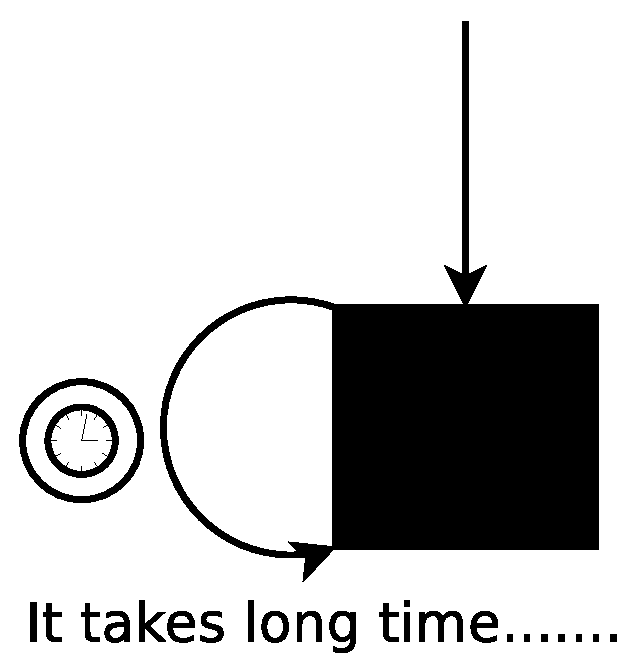
\includegraphics[width=5cm,height = 5cm]{pictures/blackbox}  
\end{figure}
\end{minipage}
\vfill
\begin{minipage}{\linewidth}
\quad \\
\end{minipage}
\end{frame}

\begin{frame}
\frametitle{Blackbox testing}
\begin{minipage}{\linewidth}
\begin{figure}  %栏内是一张图片
  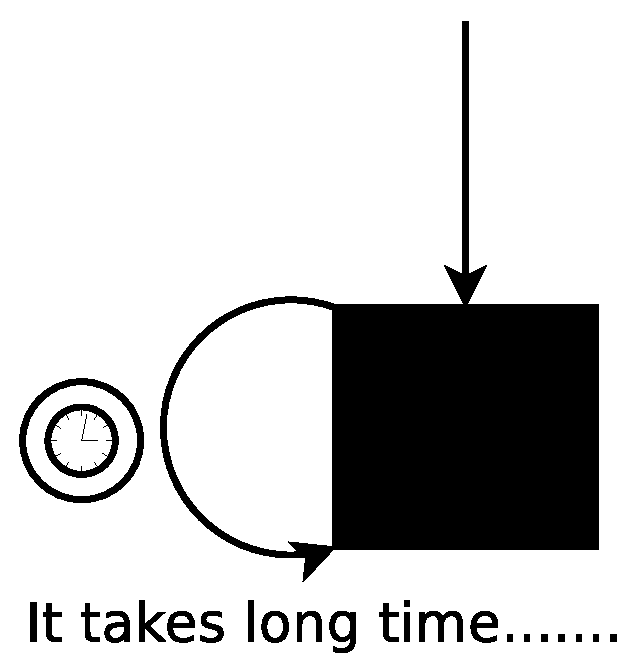
\includegraphics[width=5cm,height = 5cm]{pictures/blackbox}  
\end{figure}
\end{minipage}
\vfill
\begin{minipage}{\linewidth}
It is very important to check whether a program is \emph{\red TERMINATING} before doing the testing.
\end{minipage}
\end{frame}
\fi

\begin{frame}
\frametitle{Bad news \& Good news}
\begin{itemize}
\item In theory, \\ the termination problem of programs has been proven to be undecidable.
\item In practice, \\ just return "UNKNOWN" when we can not prove whether it is terminating.

\end{itemize}
\end{frame}

\begin{frame}
\frametitle{Bad news \& Good news}
\begin{itemize}
\item In theory, \\ the termination problem of programs has been proven to be undecidable.
\item In practice, \\ just return "UNKNOWN" when we can not prove whether it is terminating.
\end{itemize}
\hl

Goal:

\quad  For a given program, we try to avoid "UNKNOWN" result as much as possible.
\end{frame}

\begin{frame}
\frametitle{Background}
\begin{itemize}
\item It attracts many researchers to work on the termination of programs.
\item $\ultimizer$, one of the leading tools in program analysis according to the outcomes of the \textbf{\red SV-COMP} competitions.
\item The termination of \textbf{\red loops} is at the core of the termination analysis techniques used in $\ultimizer$.
\end{itemize}
\end{frame}

\iffalse
\begin{frame}[fragile]
\frametitle{General way}
\begin{minipage}{\linewidth}
\begin{lstlisting}[language=C++,
    xleftmargin=.3\textwidth, 
    xrightmargin=.3\textwidth]
while(g_1) \\Loop 1
{
  ....;
  while(g_2) \\Loop 2
  {
     ....; 
  }
  ...;
}
\end{lstlisting}
\end{minipage}
\vfill
\begin{minipage}{\linewidth}
\begin{itemize}
\item prove the termination of \textbf{\red Loop 2};
\item remove \textbf{\red Loop 2}, then prove the termination of \textbf{\red Loop 1};
\end{itemize}
\end{minipage}
\end{frame}
\fi

\begin{frame}[fragile]
\frametitle{Concern}
\begin{minipage}{\linewidth}
\begin{lstlisting}[language=C++,
    xleftmargin=.3\textwidth, 
    xrightmargin=.3\textwidth]
while(g_1) \\Loop 1
{
  ....;
  ....;
  ....;
}
\end{lstlisting}
\end{minipage}
\vfill
\begin{minipage}{\linewidth}
\begin{center}
the termination of simple loop programs, i.e., \textbf{\red no nested loops}. %with \textbf{\red simple loop}.
\end{center}
\end{minipage}
\end{frame}

\begin{frame}
\frametitle{Ranking function (RF)}
\begin{itemize}
\item Informal definition \\
\begin{center}
$f: S \rightarrow \mathbb{R}$
\end{center}
where $S$ is the set of program states, $\mathbb{R}$ is a well-founded ordered set.
\item Decrease condition \\
\begin{equation}
\forall x, x': f(x)-f(x')\geq \delta >0 \notag
\end{equation}
where $\delta \in \reals$, $x$ is current program state, $x'$ is the program state after updating.
\item Bounded condition \\
\begin{equation}
\forall x: f(x)\geq C \notag
\end{equation}
 where $C \in \reals$.
\end{itemize}
\end{frame}

\begin{frame}
\frametitle{Ranking function (RF)}
\begin{myTheorem}
A loop program P is terminating, if P has a ranking function f(x).
\end{myTheorem}
%\begin{proof}
%f(x) is decreased in every program step, and f(x) is bounded. So f(x) can only decrease in finate steps i.e. $P$ will terminate after finate updates.
%\end{proof}
\end{frame}


\begin{frame}
\frametitle{Synthesis of ranking functions}
\begin{itemize}
\item Termination of programs is undecidable.
\item Synthesis of ranking function is, however, decidable, given certain classes of ranking functions.
\end{itemize}
\end{frame}

\begin{frame}
\frametitle{Related works}
\begin{itemize}
\item \red Linear program \& Single phase linear ranking function
\begin{itemize}
\item In 2002, Col\'{o}n and Sipma synthesized linear ranking functions for linear-constraint loops. 
\item In 2004, a complete and efficient solution was proposed by Podelski and Rybalchenko.
\item ...
\end{itemize}
\item \red Linear program \& K phases ranking function 
\begin{itemize}
\item In 2005, Bradley et al. showed how to synthesize lexicographic linear ranking functions (LLRFs).
\item In 2014, Ben-Amram and Genaim provided a complete polynomial-time solution for M$\Phi$RFs with bounded depth.
\item ...
\end{itemize}
\item \red Polynomial program \& Single phase ranking function
\begin{itemize}
\item In 2005, Cousot made use of parametric abstraction and SDP to compute ranking functions of loops. 
\item In 2019, Yuan et al. proposed a ranking function detection method exploiting SVM .
\item ...
\end{itemize}
\end{itemize}
\end{frame}

\begin{frame}
\frametitle{Our contributions}
\begin{itemize}
\item Linear program \& Single phase linear ranking function
\item Linear program \& K phases ranking function 
\item Polynomial program \& Single phase ranking function
\item \textbf{\red Polynomial program} \& \textbf{\red K phases ranking function} 
\begin{itemize}
\item Based on SVM to synthesize nested ranking functions.
\item Provide the comprehensive empirical evaluation.
\end{itemize}
\end{itemize}
\end{frame}


\begin{frame}[fragile]
\frametitle{Preliminaries}
\begin{myDefinition}[Loop Program]
\label{def:loopProgram}
	A \emph{loop program} $\Omega(\varsvec, \varsvec')$ is a binary relation with free variables $\varsvec$ and $\varsvec'$, where $\varsvec$ is the current state, and $\varsvec'$ is the next state.
\end{myDefinition}
\hl
\begin{lstlisting}[language=C++,
    xleftmargin=.3\textwidth, 
    xrightmargin=.3\textwidth]
while(x>0)
{
  x++;
}
\end{lstlisting}
\begin{equation}
\Omega(\varsvec, \varsvec') \triangleq \varsvec > 0 \land \varsvec' = \varsvec + 1 \notag
\end{equation}
\end{frame}

\begin{frame}
\frametitle{Preliminaries}
\begin{myDefinition}[$k$-Nested Ranking Function]
\label{def:nestedRankingFunction}
	Given a loop program $\Omega$, let $k \in \strictlyposnaturals$ and, for each $i \in \setnocond{1, \dotsc, k}$, $\affrank_{i}(\varsvec)$ be a polynomial or an algebraic fraction over the program variables $\varsvec$. 
	We call the $k$-tuple $\langle \affrank_{1}, \affrank_{2}, \dotsc, \affrank_{k}\rangle$ a \emph{$k$-nested ranking function} of $\Omega$ if the following condition holds for a set of parameters $\setcond{C_{i} \in \strictlyposreals}{1 \leq i \leq k+1}$:
	\begin{equation}
		\forall (\varsvec,\varsvec') \in \Omega :
		\left\{
			\begin{array}{ll}
				\affrank_{1}(\varsvec) - \affrank_{1}(\varsvec') \geq C_{1} \\
				\affrank_{2}(\varsvec) - \affrank_{2}(\varsvec') + \affrank_{1}(\varsvec) \geq C_{2} \\
				\multicolumn{1}{c}{\vdots} \\
				\affrank_{k}(\varsvec) - \affrank_{k}(\varsvec') + \affrank_{k-1}(\varsvec) \geq C_{k} \\
				\affrank_{k}(\varsvec) \geq C_{k+1}
			\end{array}
		\right. \notag
		\label{eq:nestedProgress}
	\end{equation}
\end{myDefinition}
\end{frame}

\begin{frame}[fragile]
\frametitle{Example}
\begin{lstlisting}[language=C++,
    xleftmargin=.3\textwidth, 
    xrightmargin=.3\textwidth]
int q,y;
while(q>0)
{
  q = q-y;
  y = y+1;
}
\end{lstlisting}
\hl
\begin{itemize}
\item Single phase linear ranking function does not work.
\item However, it has a 2-nested ranking function.
\begin{center}
$f_1(q, y) = 1-y, f_2(q, y) = q+1, C_1 = C_2 = C_3 = 1;$
\end{center}
\end{itemize}

\end{frame}

\begin{frame}[fragile]

\frametitle{Example}
\begin{columns}

\column{.5\textwidth}

\begin{block}{Loop Program}

\begin{lstlisting}[language=C++,
    xleftmargin=.3\textwidth, 
    xrightmargin=.3\textwidth]
int q,y;
while(q>0)
{
  q = q-y;
  y = y+1;
}
\end{lstlisting}

\end{block}

\column{.5\textwidth}

\begin{block}{Phases}

\begin{figure}  %栏内是一张图片
  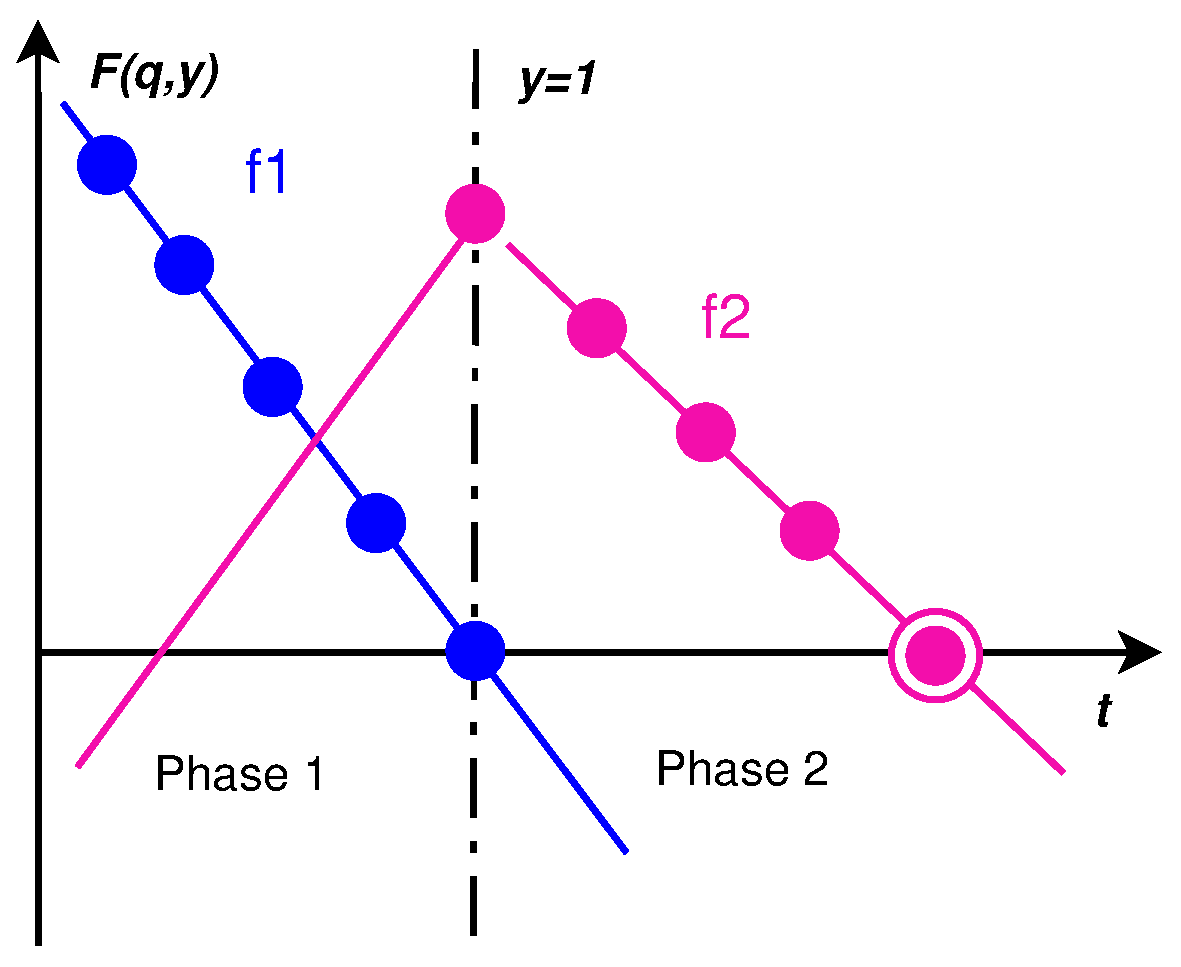
\includegraphics[width=6cm,height = 5cm]{pictures/loopPhase}  
\end{figure}
\end{block}

\end{columns}



\end{frame}

\iffalse
\begin{frame}
\frametitle{Example}
\begin{itemize}
\item Phase 1: ($y<=0$)\\
\begin{align*}
f_1: & \downarrow\\
	 & f_1(q, y)-f_1^{\ \prime}(q,y) =(1-y)-(1-(y+1)) = 1>=0; \\
f_2: & \uparrow\\
	 & f_2(q, y)-f_2^{\ \prime}(q,y) =(q+1)-(q-y+1) = y<=0; 
\end{align*}
\item Phase 2: ($y>=1$)\\
\begin{align*}
f_1: & \downarrow\\
	 & f_1(q, y)-f_1^{\ \prime}(q,y) =(1-y)-(1-(y+1)) = 1>=0; \\
f_2: & \downarrow\\
	 & f_2(q, y)-f_2^{\ \prime}(q,y) =(q+1)-(q-y+1) = y>=0; 
\end{align*}
%\item Satisfy the constraint condition\\
%\begin{align*}
%f_2(q,y)-f_2^{\ \prime}(q,y)+f_1(q,y) & \geq C_2\\
%f_2(q,y)-f_2^{\ \prime}(q,y)          & \geq C_2-f_1(q,y) 
%\end{align*}
\end{itemize}
%\begin{center}
%Whether $C_2-f_1(q,y)$ is larger than $0$? 
%\end{center}
\end{frame}
\fi

\begin{frame}
\frametitle{Intuition}
\begin{figure}  %栏内是一张图片
  \includegraphics[width=6cm,height = 5cm]{pictures/phase}  
\end{figure}
\begin{itemize}
\item We allow that the ranking function can increase in the previous phases.
\item It will finally decrease in their own phase and the following phases. 
\end{itemize}
\end{frame}

\begin{frame}
\frametitle{Overview of the Algorithm}
\begin{figure}  %栏内是一张图片
  \includegraphics[width=12cm,height = 6cm]{pictures/Structure}  
\end{figure}
\end{frame}

\begin{frame}
\frametitle{Problems}
\begin{itemize}
\item How to check the fixed point?
\item How to verify the correctness of learned ranking function?
\item How to construct the data set?
\end{itemize}
\begin{figure}  %栏内是一张图片
  \includegraphics[width=10cm,height = 4cm]{pictures/Problem}  
%  \caption*{Problem}
\end{figure}
\end{frame}

\begin{frame}
\frametitle{How to check the fixed point?}
\begin{myDefinition}[Fixed point]
\label{def:fixedPoint}
	Given a loop program specified by $\Omega$, we say that $\varsvec \in \reals^{n}$ is a \emph{fixed point} of the loop if $(\varsvec, \varsvec) \in \Omega$.
\end{myDefinition}
\end{frame}


\begin{frame}[fragile]
\frametitle{Example}
\begin{lstlisting}[language=C++,
    xleftmargin=.3\textwidth, 
    xrightmargin=.3\textwidth]
while(x>0 && y>0)
{
  x = (x+y)-y;
  y = y;
}
\end{lstlisting}
\hl
\begin{align*}
&X' = (x',y') = ((x+y)-y,y) = (x,y) = X \\
\Longrightarrow &\forall X \in \reals^{2}_{>0}, (X,X) \in \Omega \\
\Longrightarrow &\forall X \in \reals^{2}_{>0}, X\ is\ a\ fixed\ point.
\end{align*}
\end{frame}

\begin{frame}
\frametitle{How to verify the correctness of learned ranking functions?}

\begin{itemize}
%\item It is easy to check the correctness given the ranking function and the loop programs.
\item Decreased condition \& Bounded condition
\item SMT tools, like Z3, etc.
\end{itemize}

\begin{block}{Check for single phase ranking function}
\[
\forall (x,x') \in \Omega: f(x) \geq C \land f(x) - f(x') \geq \delta
\]

\end{block}

\end{frame}

\begin{frame}
\frametitle{How to verify the correctness of learned ranking functions?}

\begin{block}{Check for nested ranking functions}
	\begin{equation}
		\forall (\varsvec,\varsvec') \in \Omega :
		\left\{
			\begin{array}{ll}
				\affrank_{1}(\varsvec) - \affrank_{1}(\varsvec') \geq C_{1} \\
				\affrank_{2}(\varsvec) - \affrank_{2}(\varsvec') + \affrank_{1}(\varsvec) \geq C_{2} \\
				\multicolumn{1}{c}{\vdots} \\
				\affrank_{k}(\varsvec) - \affrank_{k}(\varsvec') + \affrank_{k-1}(\varsvec) \geq C_{k} \\
				\affrank_{k}(\varsvec) \geq C_{k+1}
			\end{array}
		\right. \notag
		\label{eq:nestedProgress}
	\end{equation}
	
\end{block}
\end{frame}

\begin{frame}
\frametitle{How to construct the data set?}
\begin{itemize}
\item Relation between the SVM \& the sampled data set.
\item Relation between the SVM \& the ranking function.
\end{itemize}
\begin{figure}  %栏内是一张图片
  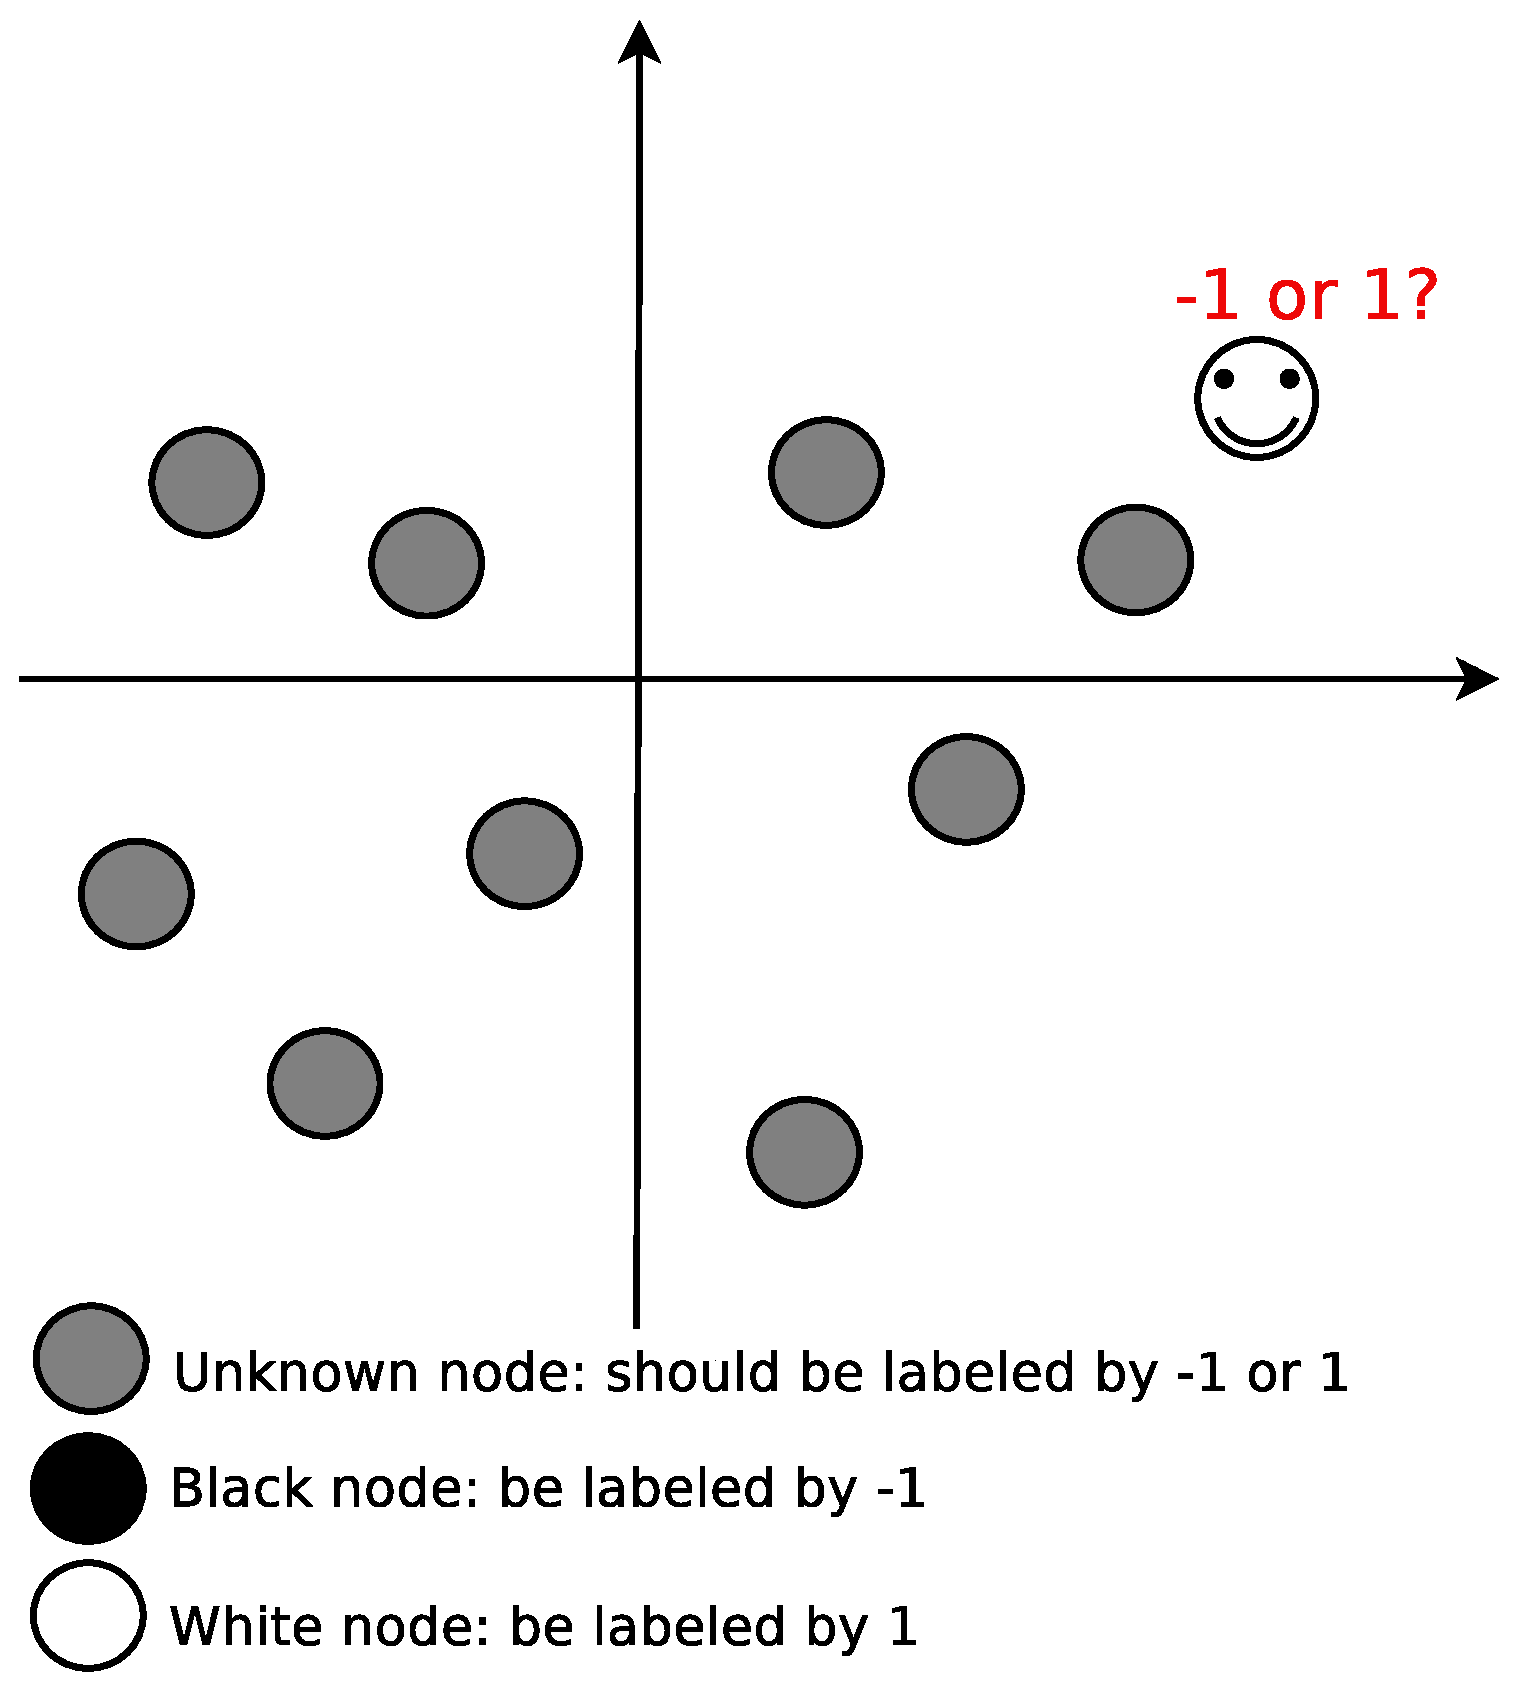
\includegraphics[width=7cm,height = 6cm]{pictures/Data}  
%  \caption*{Problem}
\end{figure}
\end{frame}
\begin{frame}
\frametitle{Ranking function}
Let $\langle \affrank_{1}, \dotsc, \affrank_{k} \rangle$ be a $k$-tuple representing a $k$-nested ranking functions; 

\begin{equation}
\affrank_{j}(\varsvec) = \vect{a}^{T}_{j} \cdot U_{j}(\varsvec) \notag
\end{equation}
where $\vect{a}_{j} = (a_{j,1}, \dotsc, a_{j,s_{j}})$ is a real vector of coefficients and $U_{j}(\varsvec) = (U_{j,1}(\varsvec), \dotsc, U_{j,s_{j}}(\varsvec))^{T}$ is an $s_{j}$-tuple with $U_{j,i}(\varsvec) = \frac{q_{j,i}(\varsvec)}{p_{j,i}(\varsvec)}$, where $q_{j,i}(\varsvec), p_{j,i}(\varsvec) \in \reals[\varsvec]$, for $i \in \setnocond{1, \dotsc, s_{j}}$.
\end{frame}
\begin{frame}
\frametitle{Ranking function}
\begin{myExample}

\begin{equation}
f_{j}(\varsvec) = 3x^2 - 4xy + \frac{5y^3}{3x^3+2y+1} + 7 \notag 
\end{equation}
\hl
\begin{equation}
f_{j}(\varsvec) = \vect{a}^{T}_{j} \cdot U_{j}(\varsvec)  \notag
\end{equation}
 where $\vect{a}^{T}_{j} = (3, -4, 5, 7)$ and $U_{j}(\varsvec) = (x^2, xy, \frac{y^3}{3x^3+2y+1}, 1)^{T}$
\end{myExample}
\end{frame}

\begin{frame}
\frametitle{Nested ranking function}
\begin{equation}
		\forall (\varsvec,\varsvec') \in \Omega :
		\left\{
			\begin{array}{ll}
				\affrank_{1}(\varsvec) - \affrank_{1}(\varsvec') \geq C_{1} \\
				\affrank_{2}(\varsvec) - \affrank_{2}(\varsvec') + \affrank_{1}(\varsvec) \geq C_{2} \\
				\multicolumn{1}{c}{\vdots} \\
				\affrank_{k}(\varsvec) - \affrank_{k}(\varsvec') + \affrank_{k-1}(\varsvec) \geq C_{k} \\
				\affrank_{k}(\varsvec) \geq C_{k+1}
			\end{array}
		\right. \notag
		\label{eq:nestedProgress}
\end{equation}
$\Longrightarrow$
\begin{equation}
\forall (\varsvec,\varsvec') \in \Omega :
\left\{
	\begin{array}{ll}
		\vect{a}^{T}_{1} \cdot (U_{1}(\varsvec) - U_{1}(\varsvec')) \geq C_{1} \\
		\vect{a}^{T}_{2} \cdot (U_{2}(\varsvec) - U_{2}(\varsvec')) + \vect{a}^{T}_{1} \cdot U_{1}(\varsvec) \geq C_{2} \\
		\multicolumn{1}{c}{\vdots} \\
		\vect{a}^{T}_{k} \cdot (U_{k}(\varsvec) - U_{k}(\varsvec')) + \vect{a}^{T}_{k-1} \cdot U_{k-1}(\varsvec)\geq C_{k} \\
		\vect{a}^{T}_{k} \cdot U_{k}(\varsvec) \geq C_{k+1}
	\end{array}
\right. \notag
\label{eq:nestedProgressAsAU}
\end{equation}
\end{frame}
\begin{frame}
\frametitle{Substitute}
\begin{equation}
	\begin{split}
		G_{1}(\varsvec, \varsvec') \mapsto 
			\begin{pmatrix}
			\vectzero\\
			\vdots\\
			\vectzero \\
			\vectzero \\
			U_{1}(\varsvec) - U_{1}(\varsvec')
			\end{pmatrix},\ 
		G_{2}(\varsvec, \varsvec') \mapsto 
			\begin{pmatrix}
			\vectzero\\
			\vdots\\
			\vectzero\\
			U_{2}(\varsvec) - U_{2}(\varsvec')\\
			U_{1}(\varsvec)
			\end{pmatrix},\ \cdots
		\\
		\cdots,\ 
		G_{k}(\varsvec, \varsvec') \mapsto
			\begin{pmatrix}
			U_{k}(\varsvec)-U_{k}(\varsvec')\\
			\ U_{k-1}(\varsvec)\\
			\vectzero\\
			\vdots\\
			\vectzero
			\end{pmatrix},\ 
		G_{k+1}(\varsvec, \varsvec') \mapsto
			\begin{pmatrix}
			U_{k}(\varsvec)\\
			\vectzero \\
			\vectzero \\
			\vdots\\
			\vectzero
			\end{pmatrix}
	\end{split} \notag
	\label{eq:notation}
\end{equation}
\end{frame}

\begin{frame}
\frametitle{Constraint}
\begin{equation}\label{eq:nestedrf:form2}
\forall (x, x') \in \Omega :
\left\{
	\begin{array}{ll}
		(\vect{a}^{T}_{k}, \cdots, \vect{a}^{T}_{1}) \cdot G_{1}(\varsvec, \varsvec') \geq C_{1} \\
		(\vect{a}^{T}_{k}, \cdots, \vect{a}^{T}_{1}) \cdot G_{2}(\varsvec, \varsvec') \geq C_{2} \\
		\multicolumn{1}{c}{\vdots} \\
        (\vect{a}^{T}_{k}, \cdots, \vect{a}^{T}_{1}) \cdot G_{k}(\varsvec, \varsvec')  \geq C_{k} \\
		(\vect{a}^{T}_{k}, \cdots, \vect{a}^{T}_{1}) \cdot G_{k+1}(\varsvec, \varsvec')  \geq C_{k+1}
	\end{array}
\right.
\end{equation}
where $C_i>0, i\in 1..k+1$.
\end{frame}

\begin{frame}
\frametitle{SVM}
\begin{itemize}
\item Positive examples:
\begin{equation}
f(x) = wx+b > 0 \notag
\end{equation}
\item Negative examples:
\begin{equation}
f(x) = wx+b < 0 \notag
\end{equation}
\end{itemize}
\begin{figure}  %栏内是一张图片
  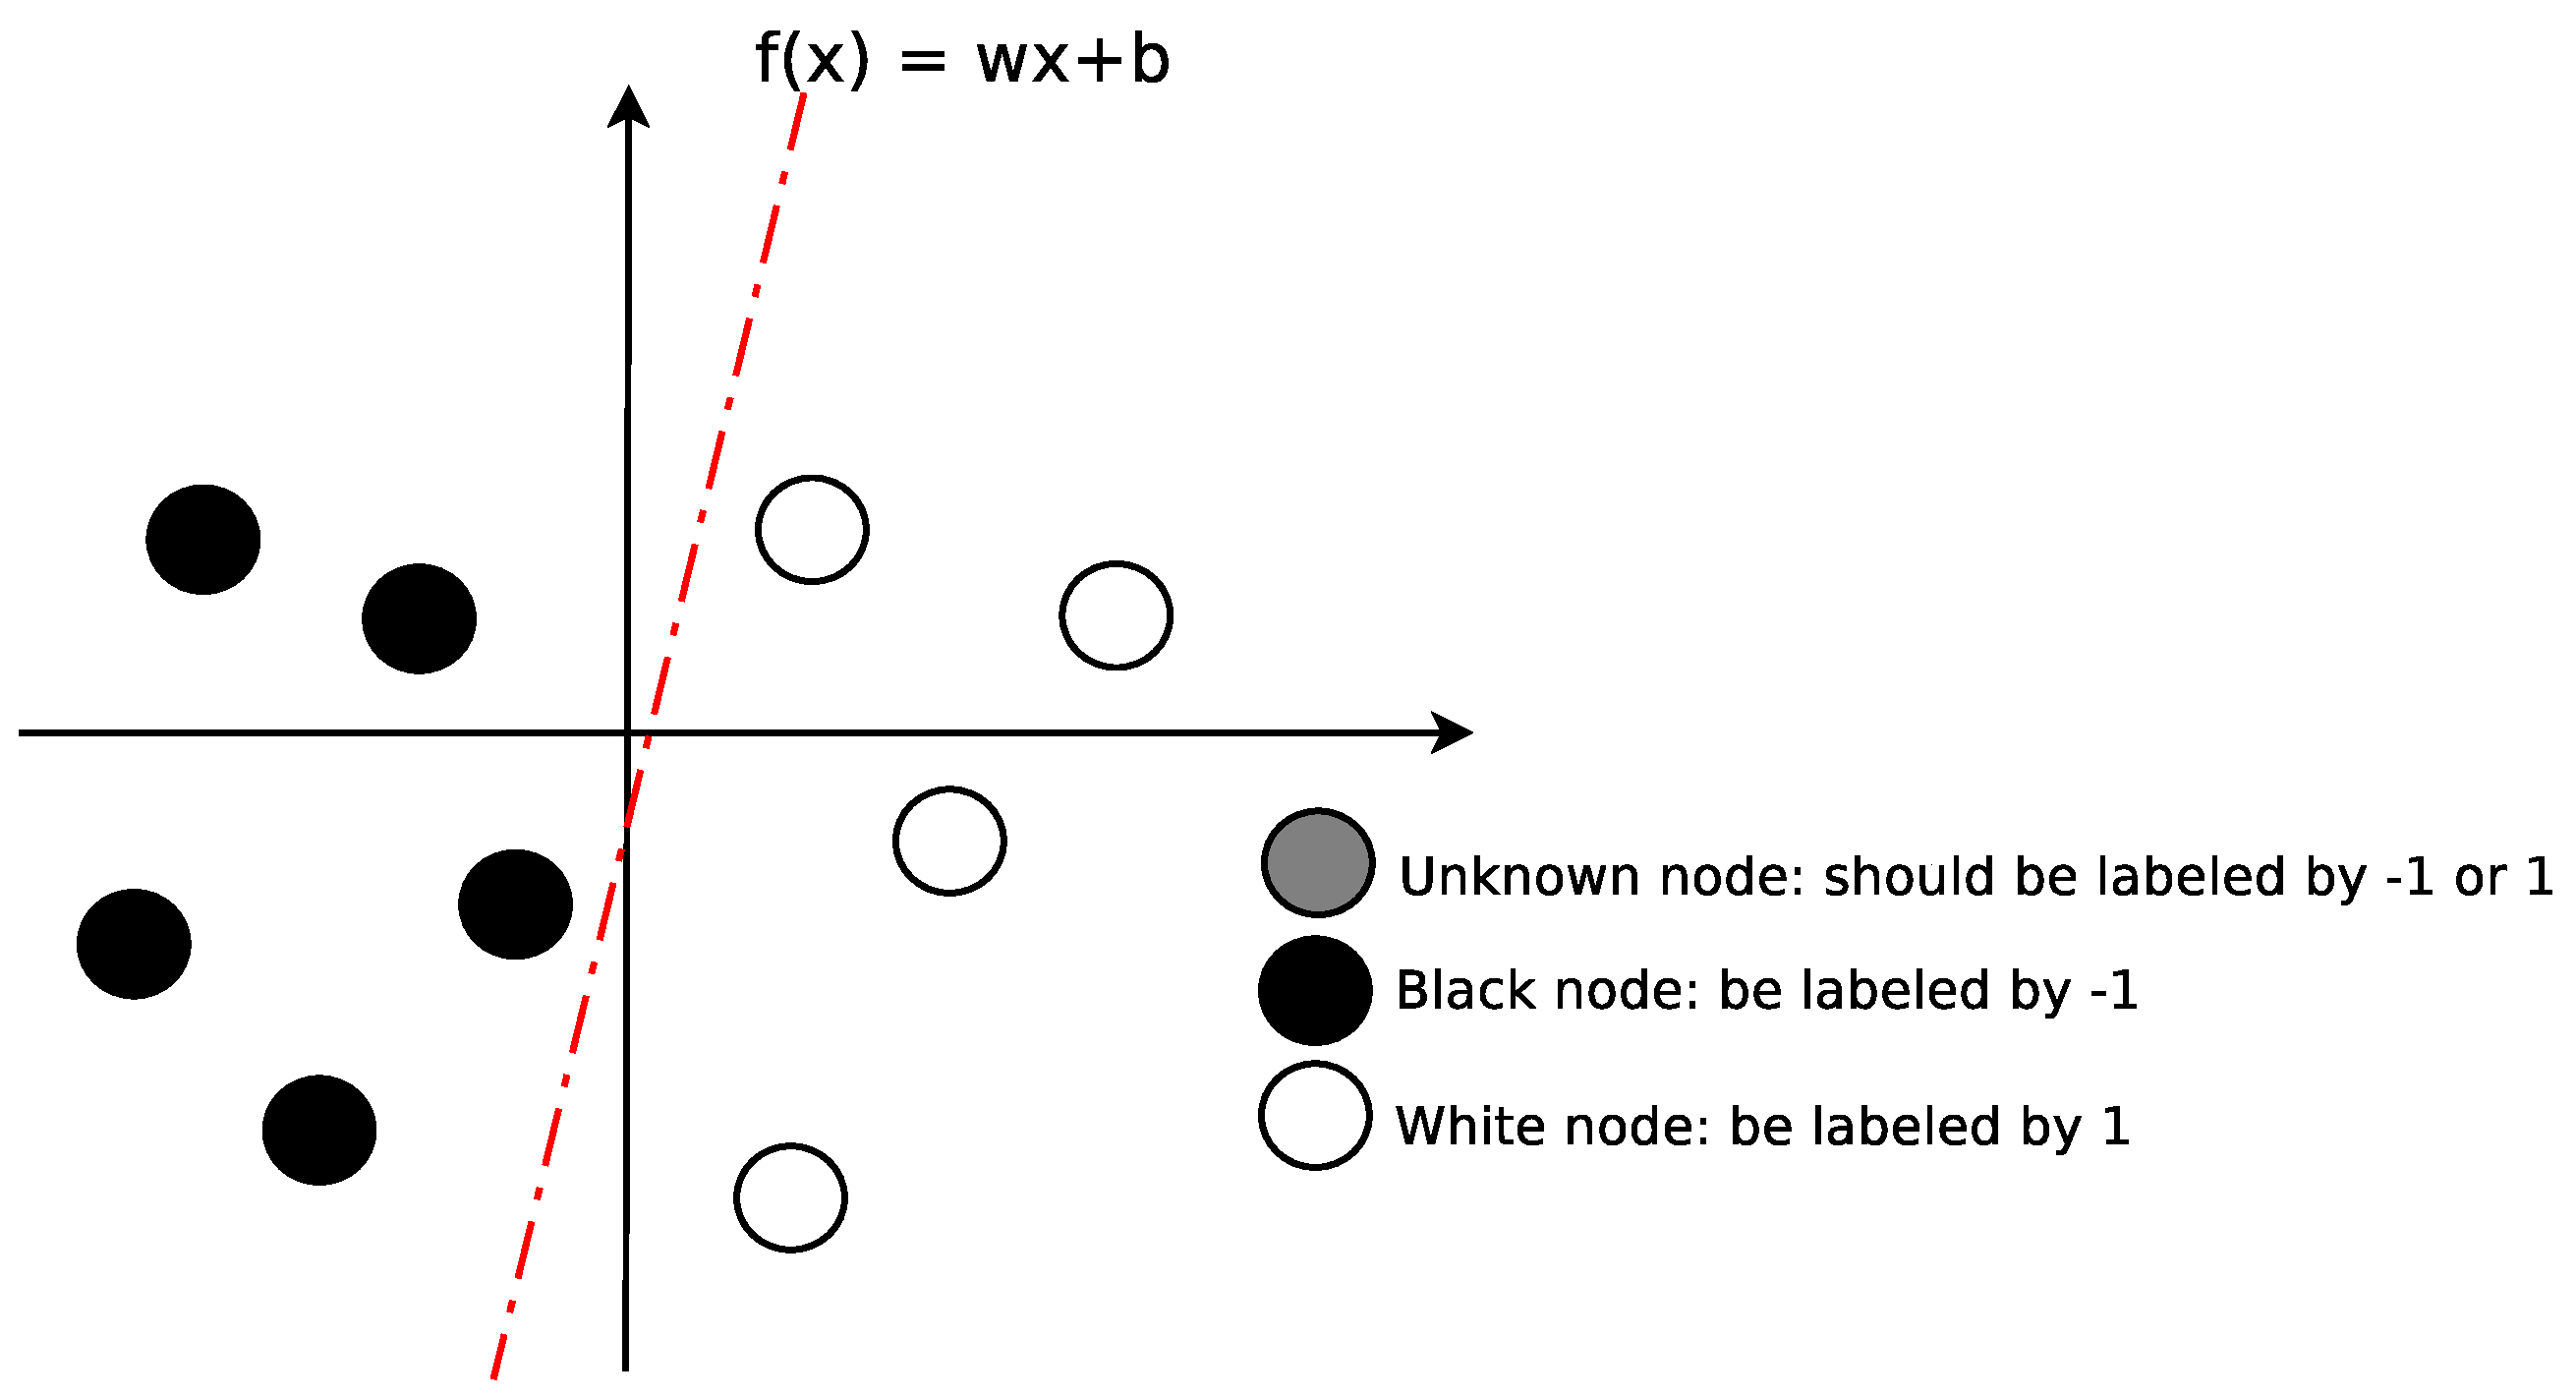
\includegraphics[width=8cm,height = 4cm]{pictures/SVM}  
%  \caption*{Problem}
\end{figure}
\end{frame}

\begin{frame}
\frametitle{Positive examples}
\begin{equation}
\forall (x, x') \in \Omega :
\left\{
	\begin{array}{ll}
		w \cdot G_{1}(\varsvec, \varsvec') +b > 0 \\
		w \cdot G_{2}(\varsvec, \varsvec') +b > 0 \\
		\multicolumn{1}{c}{\vdots} \\
        w \cdot G_{k}(\varsvec, \varsvec')  +b > 0 \\
		w \cdot G_{k+1}(\varsvec, \varsvec') +b > 0
	\end{array}
\right.\notag
\end{equation}
where $w = (\vect{a}^{T}_{k}, \cdots, \vect{a}^{T}_{1}), b = 0$.
\end{frame}

\begin{frame}
\frametitle{}
\begin{myTheorem}
\label{thm:main}
	Given a loop specified by $\Omega$, it have nested polynomial ranking functions as defined in Eq.~\ref{eq:nestedrf:form2} if and only if there exists a hyperplane $L(\vect{v})$ strictly separating the origin $\origin \in \reals^{m}$ from $G(\Omega) \subseteq \reals^{m}$.
\end{myTheorem}
\begin{proof}
\begin{figure}  %栏内是一张图片
  \includegraphics[width=5cm,height = 3cm]{pictures/proof}  
%  \caption*{Problem}
\end{figure}
\end{proof}
\end{frame}

\begin{frame}[fragile]
\frametitle{Example}
\begin{lstlisting}[language=C++,
    xleftmargin=.3\textwidth, 
    xrightmargin=.3\textwidth]
int q,y;
while(q>0)
{
  q = q-y;
  y = y+1;
}
\end{lstlisting}
\hl
\begin{center}
$f_1(q, y) = 1-y, f_2(q, y) = q+1, C_1 = C_2 = C_3 = 1;$
\end{center}
\end{frame}

\begin{frame}
\frametitle{Example}
Template 

\begin{align*}
f_1(q,y) = a_1^T \cdot U_1(q,y) = (a_{11},a_{12}, a_{13}) \cdot  (q,y,1)\\
f_2(q,y) = a_2^T \cdot U_2(q,y) = (a_{21},a_{22}, a_{23}) \cdot  (q,y,1)
\end{align*}
\hl

Constraint
\begin{equation}
\forall ((q,y),(q,y)') \in \Omega :
\left\{
	\begin{array}{ll}
		\vect{a}^{T}_{1} \cdot (U_{1}(q,y) - U_{1}(q',y')) \geq C_{1} \\
		\vect{a}^{T}_{2} \cdot (U_{2}(q,y) - U_{2}(q',y')) + \vect{a}^{T}_{1} \cdot U_{1}(q,y) \geq C_{2} \\
		\vect{a}^{T}_{2} \cdot U_{2}(q,y) \geq C_{3}
	\end{array}
\right. \notag
\end{equation}
\end{frame}

\begin{frame}
\frametitle{Substitute}
\begin{equation}
	\begin{split}
		G_{1}(q, y, q', y') \mapsto 
			\begin{pmatrix}
			\vectzero \\
			U_{1}(q, y) - U_{1}(q', y')
			\end{pmatrix},\ 
\\
		G_{2}(q, y, q', y') \mapsto 
			\begin{pmatrix}
			U_{2}(q, y) - U_{2}(q', y')\\
			U_{1}(q, y)
			\end{pmatrix},\ 
\\
		G_{3}(q, y, q', y') \mapsto
			\begin{pmatrix}
			U_{2}(q, y)\\
			\vectzero \\
			\end{pmatrix}
	\end{split} \notag
\end{equation}
\end{frame}
\begin{frame}
\frametitle{Constraint}
\begin{equation}
\forall (q, y, q', y') \in \Omega :
\left\{
	\begin{array}{ll}
		(\vect{a}^{T}_{2}, \vect{a}^{T}_{1}) \cdot G_{1}(q, y, q', y') \geq C_{1} \\
		(\vect{a}^{T}_{2}, \vect{a}^{T}_{1}) \cdot G_{2}(q, y, q', y') \geq C_{2} \\
		(\vect{a}^{T}_{2}, \vect{a}^{T}_{1}) \cdot G_{3}(q, y, q', y')  \geq C_{3}
	\end{array}
\right.\notag
\end{equation}
where $C_i>0, i\in 1..3$.
\end{frame}

\begin{frame}
\frametitle{SVM}
\begin{equation}
\forall (q, y, q', y') \in \Omega :
\left\{
	\begin{array}{ll}
		w \cdot G_{1}(q, y, q', y') +b \geq C_1 > 0 \\
		w \cdot G_{2}(q, y, q', y') +b \geq C_2 > 0 \\
		w \cdot G_{3}(q, y, q', y') +b \geq C_3 > 0
	\end{array}
\right.\notag
\end{equation}
where $w = (\vect{a}^{T}_{2}, \vect{a}^{T}_{1}), b = 0$.
\end{frame}

\begin{frame}
\frametitle{Data set}
\tikzstyle{process} = [rectangle, minimum width=3cm, minimum height=1cm, text centered, draw=black, fill = yellow!50]
\tikzstyle{file} = [draw, predproc, align=left,minimum width= 3cm, minimum height=1cm,text centered]
\tikzstyle{arrow} = [->,>=stealth]
\begin{figure}
\centering
\begin{tikzpicture}[node distance=4cm]
\node (point) [file]{Point:($\varsvec, \varsvec'$)};
\node (template)[file, below of = point, yshift = 0cm]{Template G};
\node (gx) [process, below of = point, yshift = 2cm, right of = point, xshift = 0cm]{Compute};
\node (positive) [file, right of = point, xshift = 4 cm] {positive examples  \\$G_i(\varsvec, \varsvec'), i \in 1..K+1$};
\node (negtive) [file, right of = template, xshift = 4cm] {negative examples  \\$\origin$};

\draw [arrow](point) -- (gx);
\draw [arrow](template) -- (gx);
\draw [arrow](gx) -- (positive);
\draw [arrow](gx) -- (negtive);
\end{tikzpicture}
\end{figure}
\end{frame}

\begin{frame}
\frametitle{Algorithm}
\begin{figure}  %栏内是一张图片
  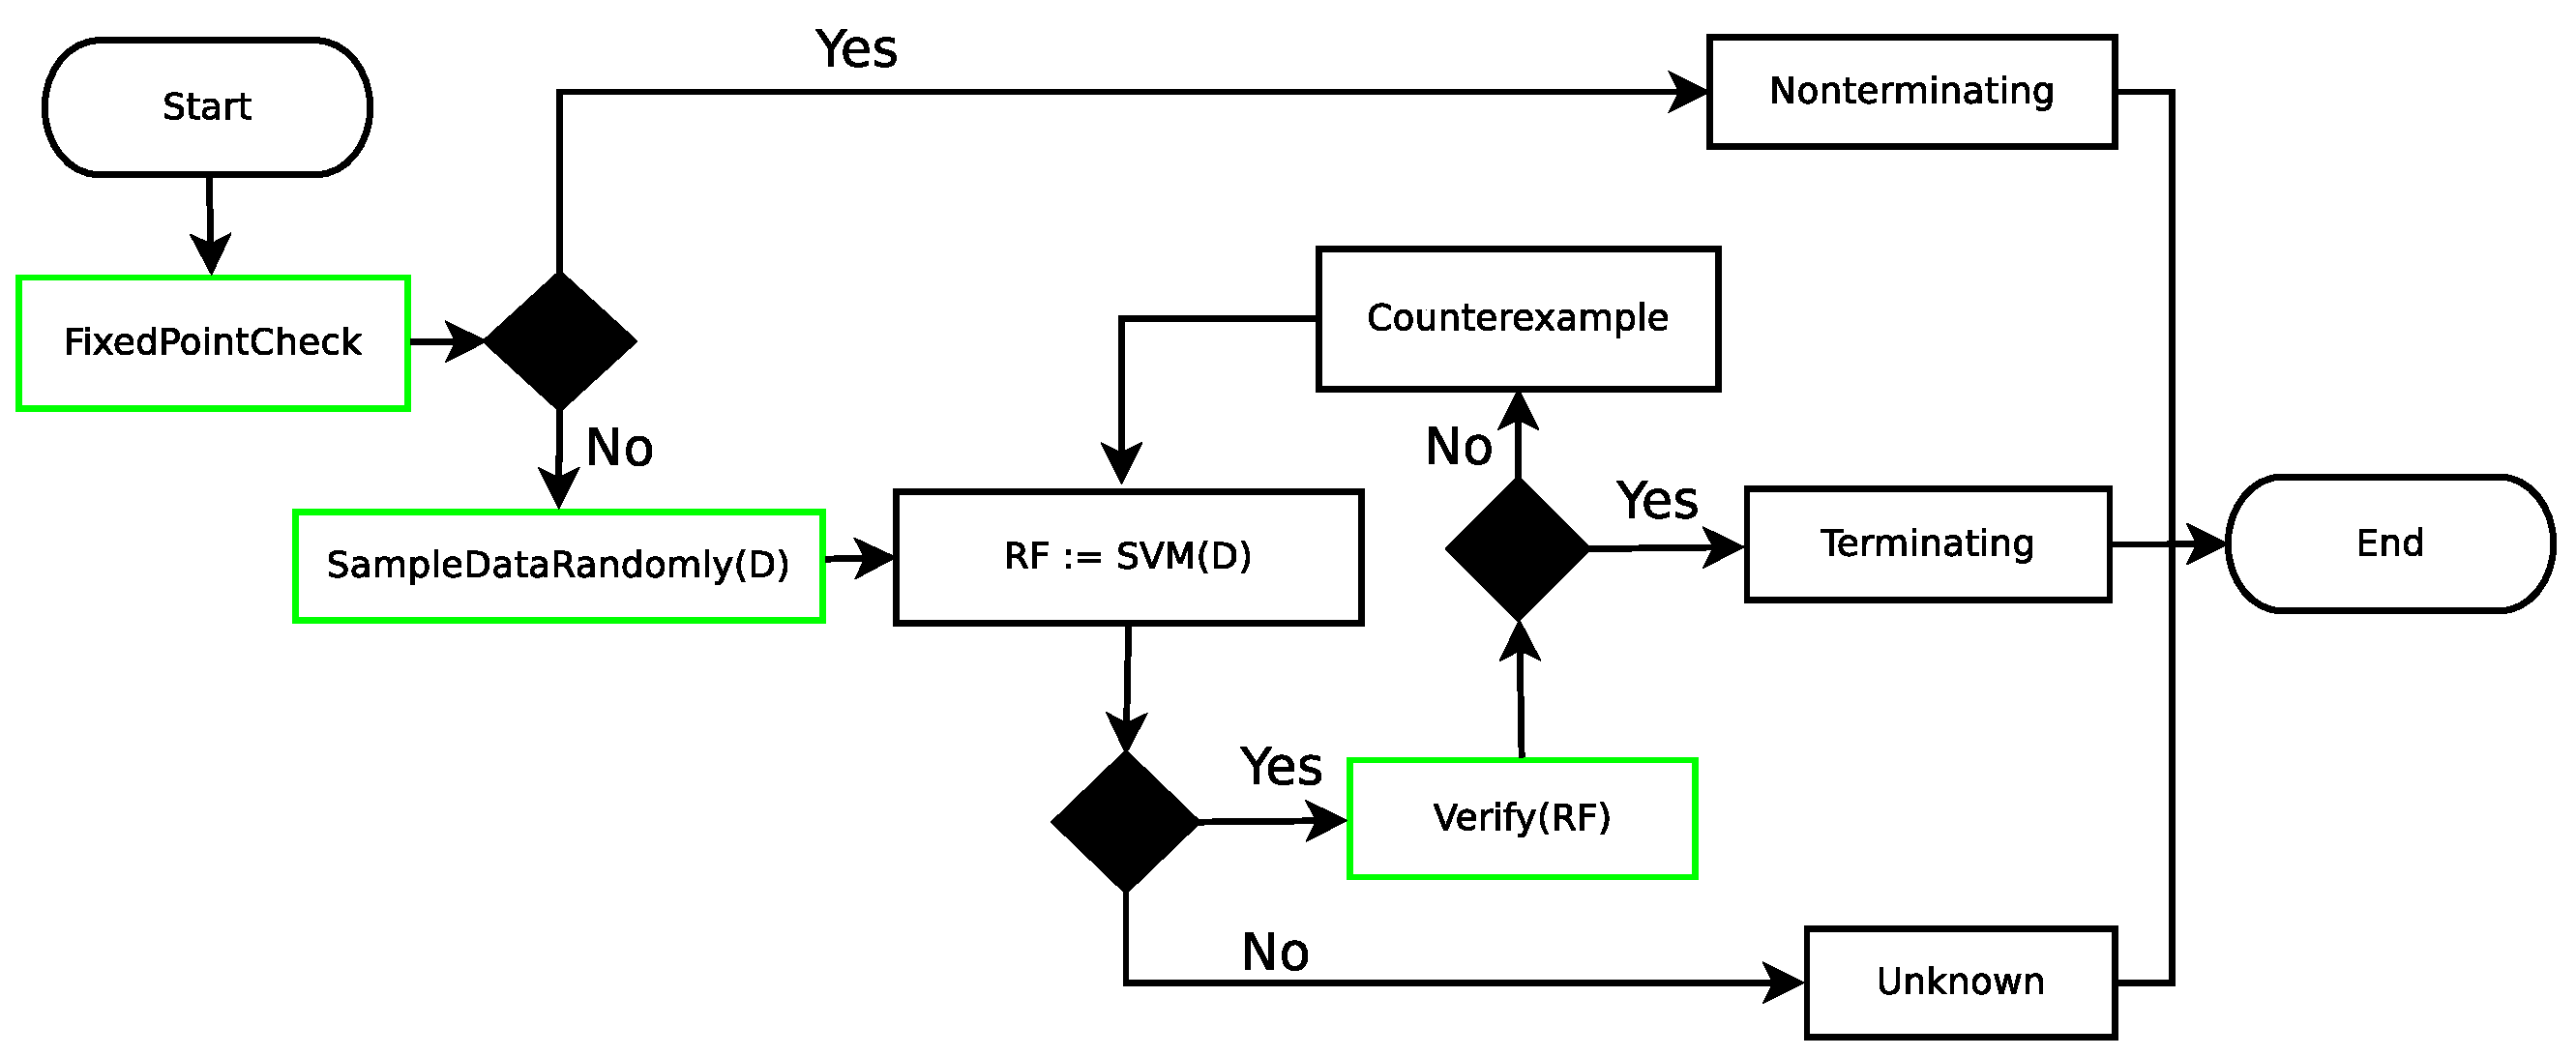
\includegraphics[width=12cm,height = 6cm]{pictures/solved}  
%  \caption*{Problem}
\end{figure}
\end{frame}

\begin{frame}
\frametitle{Algorithm}
\begin{figure}  %栏内是一张图片
  \includegraphics[width=12cm,height = 7.5cm]{pictures/algorithm}  
%  \caption*{Problem}
\end{figure}
\end{frame}



\begin{frame}
\frametitle{Experiment}
\begin{itemize}
\item Implement algorithm in a prototype tool named $\svmranker$.
\item Compare with $\lassoranker$, which is the main part of the $\ultimizer$ for proving termination of loop programs.
\item Linear program
\begin{itemize}
\item All program cases are adapted from the programs in the official website of $\lassoranker$.
\end{itemize}

\item Non-linear program
\begin{itemize}
\item All cases are adapted from the programs in related papers which focus on the termination of non-linear programs.
\end{itemize}
\end{itemize}
\end{frame}

\iffalse
\begin{frame}
\frametitle{Result}
\begin{minipage}{\linewidth}
\begin{figure}  %栏内是一张图片
  \includegraphics[width=10cm,height = 5cm]{pictures/tikz-runtime}  
\end{figure}
\end{minipage}

\begin{itemize}
\item Both tools can solve almost cases in 1s.
\end{itemize}

\end{frame}
\fi

\begin{frame}
\frametitle{Result}
\begin{table}[t]
	\label{tab:overview}
	\centering
	\begin{tabular}{c|cccc}
		 & Terminating & Non-terminating & Unknown & Timeout \\
		 \hline
		 Dataset & 65 & 69 & -& -\\
		\hline
		\svmranker & 40 & 34 & 0 & 60 \\
		\lassoranker & 24 & 37 & 73 & 0 \\
		\hline
		Common cases & 19 & 34 & 0 & 0
	\end{tabular}
	\caption{Summary of the experiments}
\end{table}
\end{frame}


\begin{frame}
\frametitle{Conclusion \& Future Work}
\begin{itemize}
\item Conclusion

\begin{itemize}
\item Based on SVM to synthesize nested ranking functions.
\begin{itemize}
\item Able to deal with the polynomial programs with nested ranking functions. 
\item Show the relation between the nested ranking functions and the SVM algorithm.
\end{itemize}
\item Provide the comprehensive empirical evaluation.
\begin{itemize}
\item Implement algorithm in a prototype tool named $\svmranker$.
\item Solve many cases with the non-linear ranking function.
\end{itemize}
\end{itemize}

\item Future Work

\begin{itemize}
\item Try to apply the learning algorithm to prove the non-termination of programs.
\item Find more efficient SMT tools to verify the ranking function.
\end{itemize}

\end{itemize}
\end{frame}

\begin{frame}
\frametitle{Experience of Master Student}
\begin{itemize}
\item Yi Li, {\red Xuechao Sun}, Yong Li, Andrea Turrini, Lijun Zhang: Synthesizing Nested
Ranking Functions for Loop Programs via SVM. ICFEM 2019: 438-454.(CCF-
C 类会议,大会报告作者)

\item Yong Li, {\red Xuechao Sun}, Andrea Turrini, Yu-Fang Chen, Junnan Xu: ROLL 1.0:
ω-Regular Language Learning Library. TACAS (1) 2019: 365-371.(CCF-B 类
会议,工具短文,大会报告作者)


\end{itemize}
\end{frame}

\begin{frame}
\begin{center}
\Large Thanks! \& Questions?
\end{center}
\end{frame}




%\end{CJK*}
\end{document}
